\chapter{Εύρωστη τοποθέτηση πόλων}\label{ch:pp}
Στο παρόν κεφάλαιο θα εξετάσουμε το πρόβλημα της εύρωστης τοποθέτησης πόλων. Η
τοποθέτηση πόλων είναι μία τεχνική ελέγχου κατά την οποία επιδιώκουμε να
ικανοποιήσουμε συγκεκριμένα επιθυμητά χαρακτηριστικά, όπως χρόνος ανύψωσης,
χρόνος αποκατάστασης, ευστάθεια κτλ. Στην περίπτωση αβέβαιων συστημάτων, η
ανάγκη ικανοποίησης των επιθυμητών χαρακτηριστικών είναι επιπλέον επιτακτική,
καθώς κάποια διαταραχή μπορεί να οδηγήσει σε έντονη απόκλιση από την επιθυμητή
κατάσταση. Η ανάπτυξη του κεφαλαίου βασίζεται στο βιβλίο~\cite{kosmidou2009robust}.

Θα μελετήσουμε το τυπικό γραμμικό αβέβαιο σύστημα της μορφής
\begin{equation}\label{eq:pp_un_ss}
    \dot{x}(t) = (A + \Delta A)x(t) + Bu(t), \quad x(t_0) = x_0,
\end{equation}
για \( t \geq t_0 \), όπου \( x(t) \in \mathbb{R}^n \) το διάνυσμα κατάστασης,
\( u(t) \in \mathbb{R}^m \) το διάνυσμα ελέγχου, \( A \) και \( B \) οι πίνακες
κατάστασης και ελέγχου αντίστοιχα, κατάλληλων διαστάσεων. Η αβεβαιότητα
περιγράφεται από τη μορφή
\[
    \Delta A = \sum_{i = 1}^{k} A_i r_i
\]
όπου \( A_i \) είναι σταθερός πίνακας και \( r_i \) βαθμωτό
μέγεθος, που μπορεί να είναι και χρονικά μεταβαλλόμενα στη γενική περίπτωση. Με
την παραπάνω περιγραφή, η παράμετρος \( r_i \) ανήκει στο σύνολο
\[
    \mathcal{R} := \{ r \in \mathbb{R}^k: |r_i| \leq \bar{r}, \bar{r} > 0, ,i = 1, \dots,
    k \}.
\]
Χωρίς να μειωθεί η γενικότητα τα όρια μπορούν να κανονικοποιηθούν, δηλαδή \(
\bar{r} =  1 \). Έτσι ονομάζουμε \emph{αποδεκτή αβεβαιότητα}, τις
αβεβαιότητες που ικανοποιούν τις γραμμικές μορφές, όπως ορίστηκαν παραπάνω, και
βρίσκονται εντός των φραγμένων συνόλων.

Όπως είδαμε στο κεφάλαιο του εγγυημένου κόστους, ο πίνακας που περιγράφει τις
αβεβαιότητες επιτρέπει, το μη μοναδικό, διαχωρισμό μοναδιαίας τάξης
\[
    A_i = d_ie_i^T,
\]
όπου \( i = 1, \dots k \) και \( d_i, e_i \in \mathbb{R}^n \). Με βάση τον
παραπάνω διαχωρισμό ορίζονται οι συμμετρικοί και θετικά ορισμένοι
πίνακες
\[
   T = \sum_{i = 1}^k d_id_i^T, \quad
   U = \sum_{i = 1}^k e_ie_i^T.
\]
Θα θεωρήσουμε τις επιδόσεις του συστήματος ότι περιγράφονται από τετραγωνική
συνάρτηση κόστους
\begin{equation}\label{eq:pp_un_cost}
    J(x_0, \Delta A, t) = \int_{t_0}^{\infty}
    \left[ x^T(t)Qx(t) + u^T(t)Ru(t) \right] \, dt.
\end{equation}
Σε πλήρη αντιστοιχία με το κεφάλαιο του εγγυημένου κόστους, για το σύστημα~\eqref{eq:pp_un_ss}
με την τετραγωνική συνάρτηση κόστους~\eqref{eq:pp_un_cost} η συνάρτηση
\( \tilde{u}:\mathbb{R} \to \mathbb{R}^m \) ονομάζεται \emph{νόμος ελέγχου εγγυημένου κόστους},
αν υπάρχει ένας θετικός αριθμός \( \tilde{J} \), που λέγεται \emph{εγγυημένο κόστος}, τέτοιος ώστε
\[
    J(x_0, \tilde{u}, \Delta A, t) \leq \tilde{J}
\]
για όλες τις αποδεκτές αβεβαιότητες. Αποδεικνύεται ότι ο γραμμικός νόμος ελέγχου
ανάδρασης κατάστασης
\[
    \tilde{u}(t) = Kx(t) = - R^{-1}B^{T}Px(t),
\]
είναι ένας νόμος ελέγχου εγγυημένου κόστους και
\[
    \tilde{J}(x_0) = x_0^{T}Px_0,
\]
είναι ένα εγγυημένο κόστος ή με κάποιες τεχνικές παραδοχές στην αντίστοιχη μορφή
\begin{equation}\label{eq:pp_un_gcc_J}
    \tilde{J} = \tr{P},
\end{equation}
αν υπάρχει ένας θετικά ορισμένος συμμετρικός πίνακας
\( P \) που ικανοποιεί τη γενικευμένη αλγεβρική εξίσωση \tl{Riccati}, για
συντομία \tl{GARE},
\begin{equation}\label{eq:pp_un_gare_general}
    PA + A^{T}P - P(BR^{-1}B^{T} - T)P + Q + U = 0.
\end{equation}
Ακόμα το σύστημα που προκύπτει είναι ασυμπτωτικά ευσταθές για κάθε αποδεκτή
αβεβαιότητα, δηλαδή για κάθε \( r_i \in \mathcal{R} \).

Όπως αναφέραμε, επιθυμούμε το σύστημα να τείνει εκθετικά στο μηδέν αλλά
επιθυμούμε να έχει το σύστημα κάποια συγκεκριμένα χαρακτηριστικά. Αυτό
μεταφράζεται, οι ιδιοτιμές του κλειστού συστήματος θέλουμε να βρίσκονται
αριστερά από κάποια επιλεγμένη τιμή, έστω \( a \), ή αντίστοιχα το κλειστό
σύστημα να έχει \emph{βαθμό σχετικής ευστάθειας} \( a \).

Για να επιτύχουμε τον προαναφερθέν βαθμό σχετικής ευστάθειας, θεωρούμε τους
μετασχηματισμούς στο πεδίο του χρόνου, \( \hat{x}(t) := e^{at}x(t) \)
και \( \hat{u}(t) := e^{at}u(t) \) και έτσι το σύστημα μετασχηματίζεται
\begin{equation}\label{eq:pp_un_a}
    \dot{\hat{x}}(t) = (A + \Delta A + aI)\hat{x}(t) + B\hat{u}(t), \quad
    \hat{x}(t_0) = \hat{x}_0 = e^{at_0}x_0,
\end{equation}
με αντικειμενική συνάρτηση όπως της σχέσης~\eqref{eq:pp_un_cost} αλλά για τις
νέες συντεταγμένες \( \hat{x} \) και \( \hat{u} \).

Με την περιγραφή αυτή το πρόβλημα μετατρέπεται σε ένα πρόβλημα εγγυημένου
κόστους που μπορεί να λυθεί με τις μεθόδους που αναφέραμε μέχρι τώρα.

Κατά το σχεδιασμό συστημάτων χωρίς αβεβαιότητες, η επιλογή των μητρώων
στάθμισης επιτρέπει τη βελτίωση των χαρακτηριστικών κλειστού βρόχου, όπως
περιθώρια ευρωστίας. Αντίστοιχα, για την περίπτωση αβέβαιων συστημάτων η
κατάλληλη επιλογή του μητρώου στάθμισης μπορεί να μας οδηγήσει στο βαθμό
σχετικής ευστάθειας που επιθυμούμε.

Έστω ότι ο συμμετρικός και θετικά ορισμένος πίνακας \( T \) μπορεί να γραφτεί
στη μορφή \( T = B\hat{T}B^T \), που ισχύει όταν οι αβεβαιότητες ικανοποιούν
τις συνθήκες προσαρμογής. Τότε η αλγεβρική εξίσωση \tl{Riccati} για το μη
αβέβαιο σύστημα γίνεται
\begin{equation}\label{eq:pp_un_wei}
    PA + A^{T}P - PB\hat{R}^{-1}B^{T} - TP + \hat{Q} = 0,
\end{equation}
όπου \( \hat{R}^{-1} = R^{-1} - \hat{T} \) και \( \hat{Q} = Q + U \). Ο νόμος
ελέγχου είναι
\[
    u(t) = -\hat{R}^{-1}B^TPx(t)
\]
και το κλειστό σύστημα γίνεται
\begin{equation}\label{eq:pp_closed}
    \dot{x}(t) = (A - B\hat{R}^{-1}B^TP)x(t) = Fx(t).
\end{equation}
Αντίστοιχα, το κλειστό αβέβαιο σύστημα περιγράφεται από
\[
    \dot{x}(t) = Fx(t).
\]
Η αλγεβρική γενικευμένη εξίσωση \tl{Riccati} της σχέσης~\eqref{eq:pp_un_gare_general}
συνδέεται με τη φασματική δομή του Χαμιλτονιανού πίνακα
\begin{equation*}
    H =
    \begin{bmatrix}
        A & -BR^{-1}B^T + T \\
        -Q - U & -A^T
    \end{bmatrix}.
\end{equation*}
Αν πάρουμε τη μορφή \tl{Jordan} του \( H \) προκύπτει
\begin{equation}\label{eq:pp_hamil}
    \begin{bmatrix}
        A & -BR^{-1}B^T + T \\
        -Q - U & -A^T
    \end{bmatrix}
    \begin{bmatrix}
        X_0 & W_0 \\
        Y_0 & Z_0
    \end{bmatrix} =
    \begin{bmatrix}
        X_0 & W_0 \\
        Y_0 & Z_0
    \end{bmatrix}
    \begin{bmatrix}
        \Lambda_s & 0 \\
        0 & \Lambda_u
    \end{bmatrix},
\end{equation}
όπου \( \Lambda_s \) και \( \Lambda_u \) είναι διαγώνιοι πίνακες των ευσταθών
(αρνητικών) και ασταθών (θετικών) ιδιοτιμών του \( H \) αντίστοιχα.

Πρέπει να αναφέρουμε ότι ο μετασχηματισμός του \( H \) σε διαγώνια μορφή ισχύει
όταν ο \( H \) έχει διακριτές ιδιοτιμές και τότε οι στήλες του πίνακα που
δημιουργείται από τους πίνακες \( X_0, W_0, Y_0, Z_0 \), είναι τα γενικευμένα
ιδιοδιανύσματα του \( H \). Επίσης, κατά την υλοποίηση του αλγορίθμου είναι προτιμότερο
ο μετασχηματισμός να γίνει μέσω των γενικευμένων ιδιοδιανυσμάτων του πίνακα
\( H \) και όχι μέσω της μορφής \tl{Jordan}. Αυτό διότι ο αλγόριθμος που
υπολογίζει τη μορφή \tl{Jordan} στο \tl{MATLAB} αλλά και σε διάφορα άλλα υπολογιστικά
πακέτα, δεν είναι ιδιαίτερα γρήγορος.  Ένα ακόμα σημείο που πρέπει να προσέξουμε
κατά την υλοποίηση του αλγορίθμου είναι ότι ζητάμε οι διαγώνιοι πίνακες
\( \Lambda_s \) και \( \Lambda_u \) να είναι τοποθετημένοι όπως παρουσιάζονται
στη σχέση~\eqref{eq:pp_hamil}, δηλαδή πρώτα οι αρνητικές και μετά οι θετικές
ιδιοτιμές. Εφόσον κατά τον υπολογισμό δεν έχουμε την επιθυμητή μορφή, είναι γνωστό
ότι με εναλλαγή στις στήλες γενικευμένων ιδιοδιανυσμάτων μπορούμε να λάβουμε την
ισοδύναμη επιθυμητή μορφή.

Αποδεικνύεται ότι αν το ζεύγος \( (A, B) \) είναι σταθεροποιήσιμο, τότε
\( P = Y_0 X_0^{-1} \) και \( FX_0 = X_0\Lambda_s \). Ακόμα, αν το ζεύγος \( (A, B) \)
είναι πλήρως ελέγξιμο, τότε ο συμμετρικός και αρνητικά ορισμένος πίνακας
\( P_u = Z_0 W_0^{-1} \) υπάρχει και είναι λύση της~\eqref{eq:pp_un_gare_general}.
Επίσης, αποδεικνύεται ότι αντικαθιστώντας τον πίνακα στάθμισης των καταστάσεων
\( Q \) με \( Q + \Delta Q \), όπου \( \Delta Q = - 2aP_u \), στη συνάρτηση κόστους,
οι ιδιοτιμές του κλειστού ονομαστικού συστήματος μετατοπίζονται κατά \( -2a \).
Η αντίστοιχη γενικευμένη εξίσωση \tl{Riccati} γίνεται
\begin{equation}\label{eq:pp_un_gare_a}
    \bar{P}(A + aI) + (A + aI)^{T}\bar{P} - \bar{P}(BR^{-1}B^{T} - T)\bar{P} +
    Q + U - 2aP_u= 0.
\end{equation}

Σύμφωνα με τα παραπάνω προκύπτει το παρακάτω θεώρημα.
\begin{theorem}[Θεώρημα 5.7 της Κοσμίδου~\cite{kosmidou2009robust}]
    Έστω \( \Lambda_s \) το φάσμα του κλειστού συστήματος~\eqref{eq:pp_closed}
    για κάποιους δεδομένους πίνακες βάρους \( Q \) και \( R \). Ακόμη, έστω οι
    εισάγεται βαθμός σχετικής ευστάθειας \( a \) και ο πίνακας βάρους
    κατάστασης \( Q \) τροποποιείται κατά
    \[
        \Delta Q = -2aP_u,
    \]
    όπου \( P_u \) είναι η αρνητικά ορισμένη λύση
    της~\eqref{eq:pp_un_gare_general}. Τότε το φάσμα \( \Lambda(\tilde{F}_s) \)
    του ονομαστικού κλειστού συστήματος με βαθμό σχετικής ευστάθειας \( a \)
    και τροποποιημένο δείκτη επιδόσεων είναι
    \[
        \Lambda(\tilde{F}_s) = \Lambda_s - 2aI.
    \]
\end{theorem}
Σύμφωνα με το παραπάνω θεώρημα εφαρμόζοντας τον νόμο ελέγχου
\[
    u(t) = -\hat{R}^{-1}B^T\bar{P}_sx(t),
\]
όπου \( \bar{P}_s \) είναι η θετικά ορισμένη λύση της
σχέσης~\eqref{eq:pp_un_gare_a}, οι ιδιοτιμές του ονομαστικού κλειστού
συστήματος μετατοπίζονται κατά \( -2a \) και αντίστοιχα οι ιδιοτιμές του
αβέβαιου συστήματος~\eqref{eq:pp_un_ss} βρίσκονται αριστερά του \( -a \) του
μιγαδικού επιπέδου, για όλες τις αποδεκτές αβεβαιότητες.

Ο παραπάνω νόμος ελέγχου προϋποθέτει την ύπαρξη λύσεων των εξισώσεων~\eqref{eq:pp_un_gare_general}
και~\eqref{eq:pp_un_gare_a}. Ακόμα οι λύσεις οι οποίες προκύπτουν δεν είναι
μοναδικές ή μπορεί ο αντίστοιχος πίνακας \tl{Riccati} να μην είναι θετικά
ορισμένος. Για το λόγο αυτό το παρόν κεφάλαιο συνοψίζεται σε έναν αλγόριθμο
τριών βημάτων, όπου επιλύουμε προβλήματα ελαχιστοποίησης \tl{LMI} ούτως ώστε το
εγγυημένο κόστος να είναι το ελάχιστο και ακόμα να ικανοποιείται ο βαθμός
σχετικής ευστάθειας.

\section{Αλγόριθμος εύρωστης τοποθέτησης πόλων}
Θα παρουσιάσουμε τα βήματα του αλγορίθμου εφαρμόζοντας ένα παράδειγμα και σε
κάθε βήμα θα παρουσιάζουμε και τον αντίστοιχο κώδικα \tl{MATLAB} που το
υλοποιεί.

Θα μελετήσουμε το σύστημα της μορφής
\[
    \dot{x}(t) = (A + \Delta A)x(t) + Bu(t), \quad x(0) = 0,
\]
όπου
\[
    A =
    \begin{bmatrix}
        0 & 1 & 0 \\
        0 & 0 & 1 \\
        1 & 2 & -1
    \end{bmatrix}, \quad
    B =
    \begin{bmatrix}
        0 \\
        0 \\
        1
    \end{bmatrix}.
\]
Σημειώνεται ότι το ονομαστικό σύστημα είναι ασταθές με ιδιοτιμές
\[
    \lambda_{1, 2, 3} = -1.8019, -0.445, 1.247.
\]
Ακόμη οι αβεβαιότητες περιγράφονται από τους πίνακες
\[
    A_1 =
    \begin{bmatrix}
        0 & 0 & 0 \\
        0 & 0 & 0 \\
        0 & 1 & 0
    \end{bmatrix}, \quad
    A_2 =
    \begin{bmatrix}
        0 & 0 & 0 \\
        0 & 0 & 0 \\
        0 & 0 & 1
    \end{bmatrix}.
\]
Για συνέπεια με τους συμβολισμούς μέχρι τώρα έχουμε ότι η διάσταση του
προβλήματος, δηλαδή η διάσταση του πίνακα \( A \) είναι \( n = 3 \) και το
πλήθος των αβεβαιοτήτων \( k = 2 \). Ένας πιθανός διαχωρισμός των αβεβαιοτήτων είναι
\[
    A_1 = d_1e_1^T =
    \begin{bmatrix}
        0 \\
        0 \\
        1
    \end{bmatrix}
    \begin{bmatrix}
        0 & 1 & 0
    \end{bmatrix}, \quad
    A_2 = d_2e_2^T =
    \begin{bmatrix}
        0 \\
        0 \\
        1
    \end{bmatrix}
    \begin{bmatrix}
        0 & 0 & 1
    \end{bmatrix}.
\]
Ακόμη ορίζουμε τους πίνακες
\[
    D = \begin{bmatrix} d_1 & \dots & d_k\end{bmatrix}, \quad
    E = \begin{bmatrix} e_1 & \dots & e_k\end{bmatrix}^T,
\]
ή αντικαθιστώντας
\[
    D =
    \begin{bmatrix}
        0 & 0 \\
        0 & 0 \\
        1 & 1
    \end{bmatrix}, \quad
    E =
    \begin{bmatrix}
        0 & 1 & 0 \\
        0 & 0 & 1
    \end{bmatrix}.
\]
Ακόμη επιλέγουμε τα μητρώα στάθμισης \( Q = I_3 \) και \( R = 1 \). Τέλος,
επιλέγουμε το βαθμό σχετικής ευστάθειας \( a = 1 \). Τα δεδομένα του
προβλήματος υλοποιούνται στη συνάρτηση \mono{pp\_data} στο \tl{MATLAB} που
παρατίθεται παρακάτω.
\eng{\lstinputlisting[language=Matlab]{src/pp_data.m}}

\subsection{Βήμα 1}
Το πρώτο βήμα του αλγορίθμου περιλαμβάνει την επίλυση ενός προβλήματος
ελαχιστοποίησης γραμμικών ανισοτήτων πινάκων
\begin{equation*}
    \begin{aligned}
        & \underset{
            (M, W, S)
        }{\mathtxt{minimize}}
        & & \tr M \\
        & \mathtxt{subject to}
        & &
        \begin{bmatrix}
            M & I \\
            I & P
        \end{bmatrix} > 0 \\
        &&&
        \begin{bmatrix}
            -W(A + aI)^T - (A + aI)W + BR^{-1}B^T
            - DSD^T & WE^T & W \\
            EW & S & 0 \\
            W & 0 & Q_0^{-1}\\
        \end{bmatrix} > 0,
    \end{aligned}
\end{equation*}
όπου έχει ένα μη κενό σύνολο εφικτών λύσεων \( (M, W, S) \) με \( M \) και \( W
\) συμμετρικοί και θετικά ορισμένοι πίνακες και \( Q_0 < Q \). Ο πίνακας \( S \)
επιλέγεται διαγώνιος
\[
    S = \diag\begin{pmatrix} \sigma_1 & \dots & \sigma_k\end{pmatrix}
\]
και περιγράφει το διαχωρισμό των αβεβαιοτήτων μέσω της σχέσης
\begin{equation}\label{eq:pp_sep}
    d_ie_i^T = \sigma_i d_i (1/\sigma_i)e_i^T, \quad i = 1, \dots ,k.
\end{equation}
Αν υπάρχει εφικτή λύση του προβλήματος τότε ο \( S \) περιγράφει το βέλτιστο
διαχωρισμό υπό την έννοια ότι το ίχνος του πίνακα \( P \) της
σχέσης~\eqref{eq:pp_un_gare_general} είναι ελάχιστο. Ακόμη ισχύει ότι \( P =
W^{-1} \).

Στο παράδειγμα η επίλυση του προβλήματος \tl{LMI} δίνει
\[
    S =
    \begin{bmatrix}
        0.1488 & 0 \\
        0 & 0.1578
    \end{bmatrix}.
\]
Παρακάτω παρατίθεται το πρώτο βήμα του αλγορίθμου όπως υλοποιήθηκε στο
\tl{MATLAB}.
\eng{\lstinputlisting[language=Matlab]{src/pp_step1.m}}

\subsection{Βήμα 2}
Εφόσον υπάρχει λύση, και άρα ο βέλτιστος διαχωρισμός \( S \) είναι
γνωστός από το πρώτο βήμα του αλγορίθμου, υπολογίζονται οι πίνακες
\( T \) και \( U \). Συγκεκριμένα, επιλέγουμε το βέλτιστο διαχωρισμό,
δηλαδή από τη σχέση~\eqref{eq:pp_sep} προκύπτει
\begin{equation}\label{eq:pp_t_u_new}
    T = \sum_{i = 1}^k \sigma_i^2 d_id_i^T, \quad
    U = \sum_{i = 1}^k (1/\sigma_i)^2 e_ie_i^T,
\end{equation}
ή για το παράδειγμα υπολογίζουμε
\[
    T =
    \begin{bmatrix}
        0 & 0 & 0 \\
        0 & 0 & 0 \\
        0 & 0 & 0.047
    \end{bmatrix}, \quad
    U =
    \begin{bmatrix}
        0 & 0 & 0 \\
        0 & 45.1914 & 0 \\
        0 & 0 & 40.138
    \end{bmatrix}.
\]

Δεδομένου του βαθμού σχετικής ευστάθειας \( a = 1 \) θέλουμε να υπολογίσουμε τη
μεταβολή του πίνακα στάθμισης των καταστάσεων, όπως περιγράφεται στο
προηγούμενο θεώρημα, από τη σχέση
\[
    \Delta Q = -2aP_u.
\]
Για να υπολογίσουμε τον όρο \( \Delta Q \) πρέπει πρώτα να βρούμε τον αρνητικά
ορισμένο πίνακα \( P_u \). Ο πίνακας αυτός συνδέεται με τον Χαμιλτονιανό
πίνακα~\eqref{eq:pp_hamil} και υπολογίζεται από
\begin{equation}\label{eq:pp_pu}
    P_u = Z_0 W_0^{-1},
\end{equation}
όπως έχουμε αναφέρει προηγουμένως.

Συνεπώς υπολογίζουμε τη μορφή \tl{Jordan} του Χαμιλτονιανού
πίνακα~\eqref{eq:pp_hamil} ή μέσω των γενικευμένων ιδιοδιανυσμάτων για
μεγαλύτερη ταχύτητα υπολογισμού, και στη συνέχεια τους όρους \( P_u \), \( \Delta
Q \) και τροποποιούμε τον πίνακα κατάστασης κατά \( \Delta Q \).
Πραγματοποιώντας τις πράξεις βρίσκουμε
\[
    P_u =
    \begin{bmatrix}
        -14.5314 & 12.5177 & -0.4171 \\
        12.5177 & -67.0584 & 10.9952 \\
        -0.4171 & 10.9952 & -9.2558 \\
    \end{bmatrix}, \quad
    \Delta Q =
    \begin{bmatrix}
        29.0628 & -25.0355 & 0.8342 \\
        -25.0355 & 134.1167 & -21.9904 \\
        0.8342 & -21.9904 & 18.5116
    \end{bmatrix},
\]
με τον πρώτο να είναι αρνητικά ορισμένος με ιδιοτιμές \( \lambda_{1, 2, 3} =
-71.7627, -12.4756, -6.6073 \) και τον δεύτερο προφανώς θετικά ορισμένο.

Ο αντίστοιχος κώδικας \tl{MATLAB} που υλοποιεί το δεύτερο βήμα του αλγορίθμου
παρατίθεται παρακάτω.
\eng{\lstinputlisting[language=Matlab]{src/pp_step2.m}}

\subsection{Βήμα 3}
Στο τρίτο βήμα του αλγορίθμου επιλύουμε και πάλι ένα πρόβλημα ελαχιστοποίησης
γραμμικών ανισοτήτων πινάκων \tl{LMI},
\begin{equation*}
    \begin{aligned}
        & \underset{
            (\bar{M}, \bar{W})
        }{\mathtxt{minimize}}
        & & \tr \bar{M} \\
        & \mathtxt{subject to}
        & &
        \begin{bmatrix}
            \bar{M} & I \\
            I & \bar{W}
        \end{bmatrix} > 0 \\
        &&&
        \begin{bmatrix}
            -\bar{W}(A + aI)^T - (A + aI)\bar{W} + BR^{-1}B^T
            & \bar{W} \\
            \bar{W} & \bar{Q}_0^{-1}\\
        \end{bmatrix} > 0,
    \end{aligned}
\end{equation*}
για κάποιο \( \bar{Q}_0 < Q + U - 2aP_u \). Το \( U \) υπολογίζεται από τη
σχέση~\eqref{eq:pp_t_u_new} μετά το πρώτο βήμα του αλγορίθμου όπου έχει βρεθεί
ο βέλτιστος διαχωρισμός και το \( P_u \) από τη σχέση~\eqref{eq:pp_pu} όπως
βρέθηκε στο δεύτερο βήμα. Αν υπάρχει μία εφικτή λύση, τότε η θετικά ορισμένη
λύση της σχέσης~\eqref{eq:pp_un_gare_a} είναι η
\[
    \bar{P} = \bar{W}^{-1},
\]
και ελαχιστοποιεί το αντίστοιχο εγγυημένο κόστος.

Στο παράδειγμα η επίλυση του προβλήματος \tl{LMI} δίνει
\[
    \bar{P} = P^* =
    \begin{bmatrix}
        43.5181 & 43.3284 & 10.6657 \\
        43.3284 & 53.8495 & 16.5335 \\
        10.6657 & 16.5335 &  5.8922
    \end{bmatrix},
\]
όπου είναι θετικά ορισμένη λύση και η τιμή της αντικειμενικής συνάρτησης είναι
\[
    J^* = \tr P^* = 103.2598.
\]

Παρακάτω παρατίθεται το τρίτο βήμα του αλγορίθμου όπως υλοποιήθηκε στο
\tl{MATLAB}.
\eng{\lstinputlisting[language=Matlab]{src/pp_step3.m}}

Ακόμη στην περίπτωση του ονομαστικού συστήματος, δηλαδή όταν δεν έχουμε
αβεβαιότητες τότε κάποια βήματα του αλγορίθμου είναι περιττά και για αυτό η
περίπτωση αυτή υλοποιήθηκε σε διαφορετική συνάρτηση, αλλά εφαρμόζοντας τον
αλγόριθμο της εύρωστης τοποθέτησης πόλων. Έτσι όπως θα δούμε παρακάτω, οι
ιδιοτιμές του κλειστού συστήματος στο ονομαστικό σύστημα θα είναι αριστερά του
\( -2a \) του μιγαδικού επιπέδου, όπου \( a \) ο βαθμός σχετικές ευστάθειας.
\eng{\lstinputlisting[language=Matlab]{src/pp_nominal.m}}

Τέλος, παρατίθεται ο συνολικός αλγόριθμος στο \tl{MATLAB} όπου ενώνει τα
προηγούμενα βήματα για την εξαγωγή των αποτελεσμάτων και είναι η συνάρτηση που
χρειάζεται κάποιος να τρέξει ώστε να εφαρμόσει τον αλγόριθμο του κεφαλαίου.
\eng{\lstinputlisting[language=Matlab]{src/pp_algorithm.m}}

Στα σχήματα~\ref{fig:pp_ex1},\ref{fig:pp_ex2} και~\ref{fig:pp_ex3} παρουσιάζονται οι
καταστάσεις για το ονομαστικό σύστημα και για διάφορες τιμές των αβεβαιοτήτων καθώς
και ο νόμος ελέγχου εγγυημένου κόστους, για βαθμό σχετικής ευστάθειας \( a = 1
\), όπως προκύπτει για αρχικές συνθήκες \( x = [3, -2, 2]^T \).
\begin{figure}[h]
    \centering
    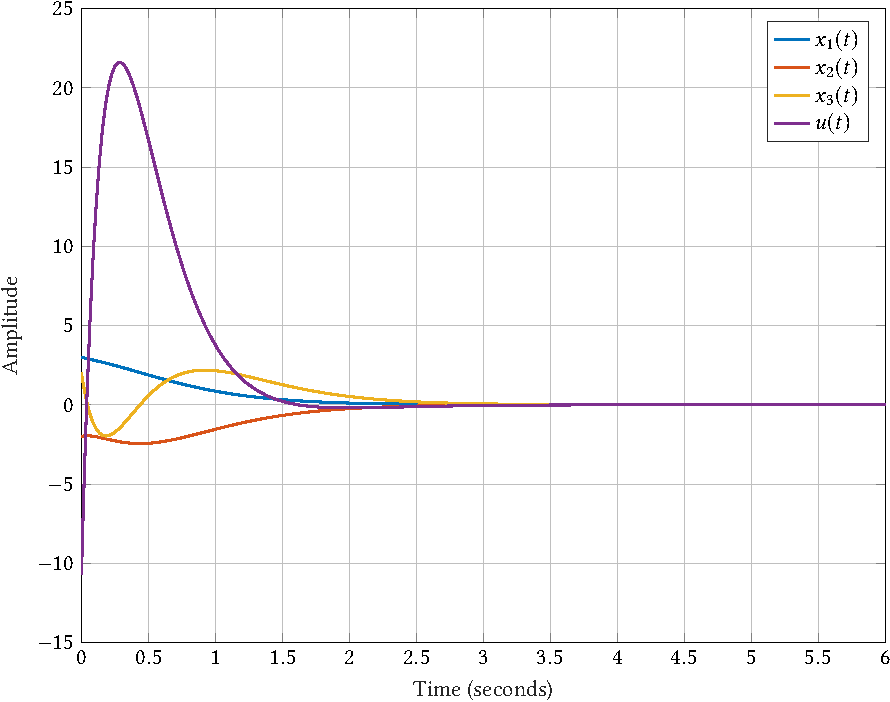
\includegraphics[width=0.9\textwidth]{figures/pp_ex1.pdf}
    \captionG{Ονομαστικό σύστημα, \( r_1 = 0, r_2 = 0, a = 1 \)}
    \label{fig:pp_ex1}
\end{figure}
\begin{figure}[h]
    \centering
    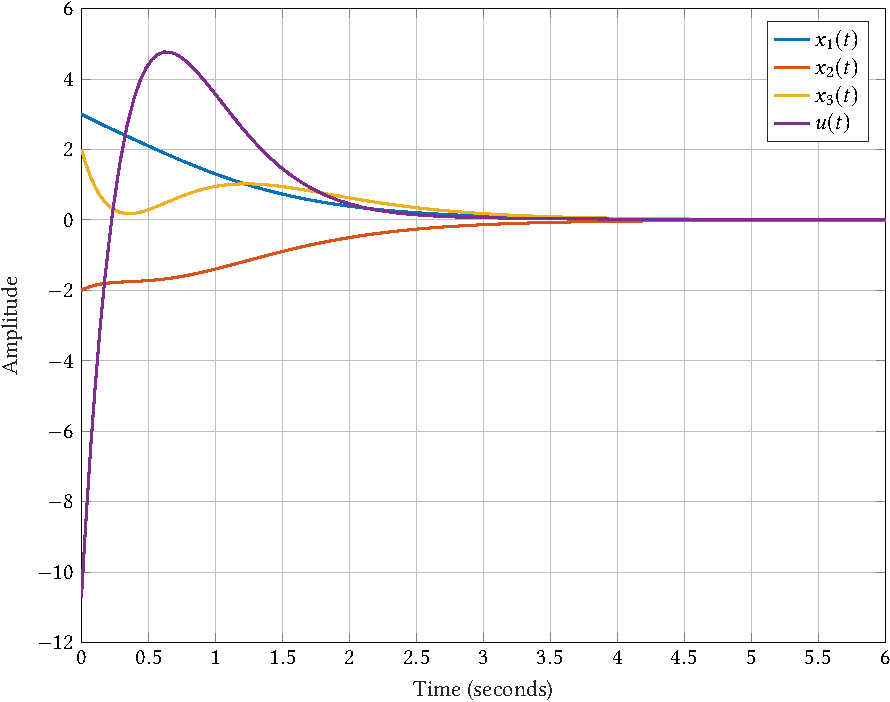
\includegraphics[width=0.9\textwidth]{figures/pp_ex2.pdf}
    \captionG{Σύστημα με αβεβαιότητες, \( r_1 = 1, r_2 = 1, a = 1 \)}
    \label{fig:pp_ex2}
\end{figure}
\begin{figure}[h]
    \centering
    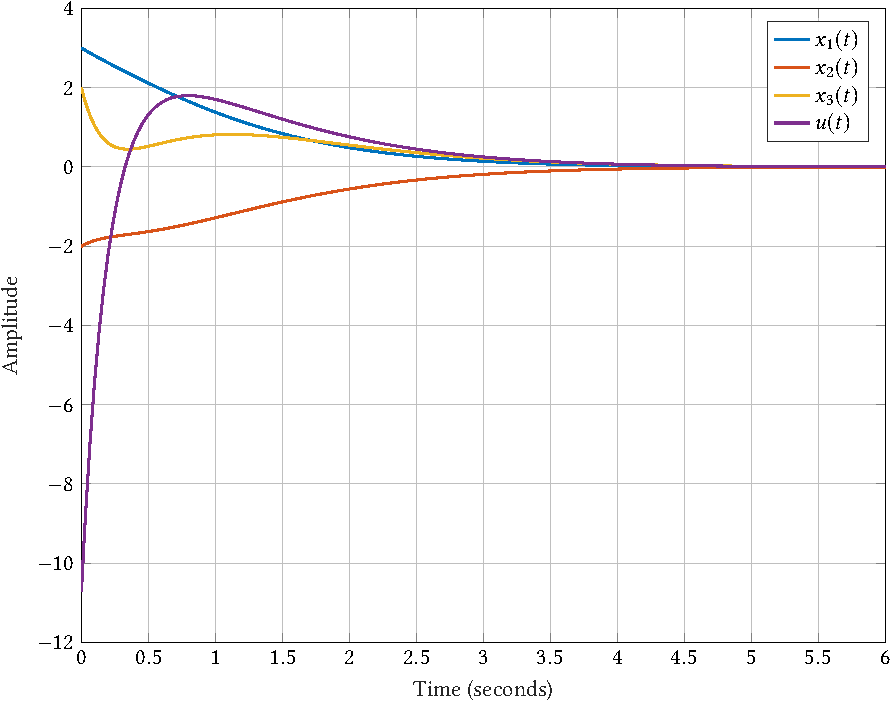
\includegraphics[width=0.9\textwidth]{figures/pp_ex3.pdf}
    \captionG{Σύστημα με αβεβαιότητες, \( r_1 = -1, r_2 = -1, a = 1 \)}
    \label{fig:pp_ex3}
\end{figure}

Στον πίνακα~\ref{tab:pp_eig_table_1} παρουσιάζονται οι ιδιοτιμές του κλειστού
συστήματος και συγκεκριμένα το πραγματικό μέρος αυτών, για διάφορες τιμές των
αβεβαιοτήτων. Ο βαθμός σχετικής ευστάθειας έχει επιλεχθεί \( a = 1 \), και
παρατηρούμε ότι ο στόχος έχει επιτευχθεί διότι όλες οι ιδιοτιμές του κλειστού
αβέβαιου συστήματος στο μιγαδικό επίπεδο βρίσκονται αριστερά του \( a \). Συνεπώς,
με τον αλγόριθμο του παρόντος κεφαλαίου, καταφέραμε όχι μόνο να σταθεροποιήσουμε το
ονομαστικό σύστημα που είναι ασταθές, αλλά καταφέραμε να τοποθετήσουμε τους πόλους
πέρα από το επιθυμητό όριο που επιλέξαμε. Ακόμα πρέπει να σημειωθεί ότι στην
περίπτωση του ονομαστικού συστήματος, όταν δηλαδή δεν έχουμε αβεβαιότητες \(
r_1 = r_2 = 0 \), τότε μέσω του αλγορίθμου οι ιδιοτιμές του κλειστού συστήματος
μετατοπίζονται αριστερά του \( -2a = -2 \) όπως παρατηρείται και τον
πίνακα~\ref{tab:pp_eig_table_1}.
\begin{table}[h]
    \centering
    \eng{\[
            \begin{tabu}{ c | c | c | c | c | c | c}
                {} & r_1 = r_2 = 0 & r_1 = r_2 = -1 & r_1 = r_2 = 1
                & r_1 = 1, r_2 = -1 & r_1 = 0, r_2 = -1 & r_1 = 1, r_2 = 0 \\
                \hline
                \lambda_1 & -2.6622 & -5.3094 & -1.2506 & -5.866 & -5.6079 & -1.3281 \\
                \lambda_2 & -3 & -1.2914 & -2.3208 & -1.0131 & -1.1421 & -1.3281 \\
                \lambda_3 & -4.1358 & -1.2914 & -2.3208 & -1.0131 & -1.1421 & -4.236 \\
            \end{tabu}
    \]}
    \captionG{Πραγματικά μέρη ιδιοτιμών κλειστού συστήματος για διάφορες
    αβεβαιότητες και \( a = 1 \)}
    \label{tab:pp_eig_table_1}
\end{table}

Σαν έναν επιπλέον έλεγχο του αλγορίθμου τρέξαμε το πρόγραμμα για διαφορετικό βαθμό
σχετικής ευστάθειας \( a = 3 \) και παραθέσαμε τον αντίστοιχο πίνακα των
ιδιοτιμών του κλειστού αβέβαιου συστήματος. Έτσι προκύπτει ο
πίνακας~\ref{tab:pp_eig_table_2}. Παρατηρούμε ότι ο αλγόριθμος τοποθέτησε τις
ιδιοτιμές αριστερά του \( -a = -3 \) στην περίπτωση που υπάρχουν αβεβαιότητες
και αριστερά του \( -2a = -6 \) για την περίπτωση του ονομαστικού συστήματος.
\begin{table}[h]
    \centering
    \eng{\[
            \begin{tabu}{ c | c | c | c | c | c | c}
                {} & r_1 = r_2 = 0 & r_1 = r_2 = -1 & r_1 = r_2 = 1
                & r_1 = 1, r_2 = -1 & r_1 = 0, r_2 = -1 & r_1 = 1, r_2 = 0 \\
                \hline
                \lambda_1 & -6.6622 & -3.6898 & -3.3941 & -3.5145 & -3.5998 & -4.1965 \\
                \lambda_2 & -7 & -3.6898 & -6.6996 & -3.5145 & -3.5998 & -4.1965 \\
                \lambda_3 & -8.1358 & -11.4138 & -6.6996 & -11.7642 & -11.5938 & -9.4002 \\
            \end{tabu}
    \]}
    \captionG{Πραγματικά μέρη ιδιοτιμών κλειστού συστήματος για διάφορες
    αβεβαιότητες και \( a = 3 \)}
    \label{tab:pp_eig_table_2}
\end{table}
\begin{table}[h]
    \centering
    \eng{\[
            \begin{tabu}{ c | c | c | c | c | c | c}
                {} & r_1 = r_2 = 0 & r_1 = r_2 = -1 & r_1 = r_2 = 1
                & r_1 = 1, r_2 = -1 & r_1 = 0, r_2 = -1 & r_1 = 1, r_2 = 0 \\
                \hline
                \lambda_1 & -20.6622 & -14.497 & -15.7631 & -14.4131 & -14.4548
                & -15.5262 \\
                \lambda_2 & -21      & -14.497 & -20.2793 & -14.4131 & -14.4548
                & -15.5262 \\
                \lambda_3 & -22.1358 & -33.8695 & -24.821 & -34.0372 & -33.9538
                & -30.8111 \\
            \end{tabu}
    \]}
    \captionG{Πραγματικά μέρη ιδιοτιμών κλειστού συστήματος για διάφορες
    αβεβαιότητες και \( a = 10 \)}
    \label{tab:pp_eig_table_3}
\end{table}
Φυσικά πρέπει να σημειωθεί ότι δε μπορούμε να επιλέξουμε αυθαίρετα το βαθμό
σχετικής ευστάθειας \( a \) διότι αυτό έχει ως αποτέλεσμα την αύξηση του
κόστους. Συγκεκριμένα, για την περίπτωση του παραδείγματος όπου επιλέξαμε \( a
= 3 \) το βέλτιστο κόστος, υπό την έννοια του αλγορίθμου, έγινε \( J^* =
5.916 \cdot 10^3 \).

Ακόμα αν για παράδειγμα επιλέξουμε το βαθμό σχετικής
ευστάθειας \( a = 10 \), προκύπτει ο πίνακας~\ref{tab:pp_eig_table_3}, τότε παρόλο που
ικανοποιούνται τα κριτήρια που θέσαμε, δηλαδή οι ιδιοτιμές βρίσκονται αριστερά
του \( -10 \) για το αβέβαιο σύστημα και αριστερά του \( -20 \) για το ονομαστικό,
το βέλτιστο εγγυημένο κόστος φτάνει την τιμή \( J^* = 3.0391 \cdot 10^6 \).
Το αν είναι αποδεκτή μία τέτοια τιμή έχει να κάνει με την υπό μελέτη εφαρμογή.
Στην παρούσα φάση η πιθανόν ακραία αυτή τιμή χρησιμοποιήθηκε απλώς για τον ελέγχο της
ορθότητας του αλγορίθμου.

Τέλος, για πληρότητα στην εργασία παραθέτουμε τους αλγορίθμους που υλοποιήθηκαν
στο \tl{MATLAB} ώστε να εξαχθούν τα αντίστοιχα διαγράμματα και οι πίνακες.
\eng{\lstinputlisting[language=Matlab]{src/pp_makeplot.m}}
